% !TeX root = ../mthesis.tex
% !TeX encoding = UTF-8
% !TeX spellcheck = en_US

\chapter{Algorithms and Data Structures}

\section{Sets of Clauses}

\subsection{Terms, Atoms, and Literals}

The recursive definition of the syntax of terms, atoms and literal suggest a tree structure.

\begin{tikzpicture}[->,>=stealth',level/.style={sibling distance = 2cm/#1,
	level distance = 0.8cm}] 

\node { $\lnot$ }
	child { 
		node { $\mP$ }
		child { node {$x$} }
		child { node {$\mf$} 
			child { node {$x$} }
		}
	}
;



\end{tikzpicture}

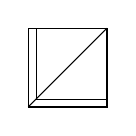
\begin{tikzpicture}
\draw (0,0) rectangle (1,1);
\draw (0.1,0.1) rectangle (1cm,1cm);

\draw (0,0) to (1,1);
\end{tikzpicture}

\subsection{Sets}

Clauses are multiset of literals.


\section{Saturation}

In the previous chapter we just applied derivation rules
on pairs of clauses chosen haphazardly from the set of clauses 
to derive and add new clauses 
until we could conclude unsatisfiability of the set of clauses.

In practice such a human approach may fail for an unsatisfiable set of clauses 
just because an important clause pairing has been overlooked 
and infinite inferences can be drawn from a satisfiable subset of the set of clauses.
%For an automated procedure we need a process that guarantees that eventually all possible inferences were drawn. 
In any case an automated procedure has to notice when all derivations have already been processed.

First will discuss the given clause algorithm in this section
as a saturation process that eventually determines all possible derivate clauses
with respect to a given calculus, e.g. ordered resolution.

\subsection{Given Clause Algorithm}

\begin{procedure}[Given Clause Algorithm]
	We start with a set of clauses $S = P \disjointunion U$, 
	where $P$ is a set of {\myem passive} clauses 
	and $U$ is the initially empty set of {\myem active} (or used) clauses.
	\begin{enumerate}
		\item[\jek] Whenever we can conclude unsatisfiability of $S$ 
		we exit the procedure with $\lnot\SAT$.
		\setcounter{enumi}{0}
		\item If $P$ is empty we exit and return \SAT.
		\item We select a passive clause, i.e.~the given clause. \jek
		\item We iterate over the active clauses and check for applicable inference rule
		for each pair of an active and the given clause
		to derive additional clauses which we add to the set of passive clauses. \jek
		\item We move the given clause from passive to active and continue with step 1.
	\end{enumerate}
\end{procedure}


In the following examples the given clause is boxed, 
the active clauses are on the left of the given clause, 
and the passive clauses are on the right. 
Each line represents one iteration of our procedure 3.
%
In both examples we start with the unsatisfiable set of clauses $S=\{\, \mP(\ma)\lor\mQ(a), \mP(\ma)\lor\lnot\mQ(y), \lnot\mP(x) \,\}$.

\subsubsection{Ordered Resolution}

\jek$\ \Leftarrow\emptyclause\in S_i$. We conclude unsatisfiability of $S$ whenever the empty clause is found (already present or derived).
New clauses are disjunctions of instances of an active and the given clause where conflicting literals were removed, 
in other words the union of the two instances without the contradicting literals.
\begin{gather*}
\infer[\sigma=\{ x'\mapsto\mf(x), y\mapsto\mg(y') \}]{
	(\mcC \lor \mcD)\sigma
}{
	\mP(\mf(x), y) \lor \mcC & \lnot\mP(x',\mg(y')) \lor \mcD
}
\end{gather*}

\begin{example}[Ordered Resolution] We assume $\mP(\ma)\succ\mQ(\ma)$,
	underline the maximal literal the given clauses,
	color conflicts red,
	 and derive the empty clause in the fifth iteration.
	
	\begin{align*}
	^{1:}&\boxed{\underline{\mP(\ma)}\lor\mQ(a)} 
	& ^{2:}&\mP(\ma)\lor\lnot\mQ(y) & ^{3:}&\lnot\mP(x) 
	\\
	^{1:}&\mP(\ma)\lor\mQ(a) 
	& ^{2:}&\boxed{\underline{\mP(\ma)}\lor\lnot\mQ(y)} & ^{3:}&\lnot\mP(x) 
	\\
	^{1:}&{\colLo\mP(\ma)}\lor\mQ(a) 
	& ^{2:}&{\colLo\mP(\ma)}\lor\lnot\mQ(y) 
	& ^{3:}&\boxed{\underline{\lnot\mP(x)}} 
	& ^{1,3:}&\mQ(\ma) 
	& ^{2,3:}&\lnot\mQ(y)
	\\
	^{1:}&\mP(\ma)\lor\mQ(a) 
	& ^{2:}&\mP(\ma)\lor{\colLo\lnot\mQ(y)} 
	& ^{3:}&\lnot\mP(x)
	& ^{1,3:}&\boxed{\underline{\mQ(\ma)}} 
	& ^{2,3:}&\lnot\mQ(y) 
	& ^{2,(1,3):}&\mP(\ma)
	\\
	^{1:}&\mP(\ma)\lor{\colLo\mQ(a)} 
	& ^{2:}&\mP(\ma)\lor\lnot\mQ(y) 
	& ^{3:}&\lnot\mP(x)
	& ^{1,3:}&\colLo\mQ(\ma) 
	& ^{2,3:}&\boxed{\underline{\lnot\mQ(y)}} 
	& ^{2,(1,3):}_{1,(2,3):}&\mP(\ma)
	& ^{(1,3),(2,3):}&\emptyclause
	\\
	\end{align*}
\end{example}

\subsubsection{InstGen}

\jek$\ \Leftarrow \lnot\SAT(S_i\bot)$. We conclude unsatisfiability of $S$ whenever (a subset of) $S_i\bot$ -- a set of ground instances -- is unsatisfiable. 
We consider only proper instances of an active and the given clause as probable new clauses to extend the set of clauses.
\begin{gather*}
	\infer[\sigma=\{ x'\mapsto\mf(x), y\mapsto\mg(y') \}]{
		\mP(\mf(x),\mg(y')) \lor\mcC\sigma 
		\qquad 
		\lnot\mP(\mf(x),\mg(y'))\lor\mcD\sigma
	}{
		\mP(\mf(x), y) \lor \mcC & \lnot\mP(x',\mg(y')) \lor \mcD
	}
\end{gather*}


\begin{example}[InstGen]The active and given clauses are already encoded and given to a \SAT solver.
	The basic given clause algorithm would stop and fail after $(4)$
	since $S_4\bot$ is still satisfiable and there is no conflict between the underlined selected literal of the given clause 
	and any selected literals of any of the active clauses.
	
	
	\begin{align*}
	(1)\quad^{1:}&\boxed{\underline{\mP(\ma)}\lor\mQ(\ma)} 
	& ^{2:}&\mP(\ma)\lor\lnot\mQ(\consbot/y) 
	& ^{3:}&\lnot\mP(\consbot/x)
	\\
	(2)\quad^{1:}&{\colHi\underline{\mP(\ma)}}\lor\mQ(\ma) 
	& ^{2:}&\boxed{\underline{\mP(\ma)}\lor\lnot\mQ(\consbot/y)} 
	& ^{3:}&\lnot\mP(\consbot/x) 
	\\
	(3)\quad^{1:}&{\colHi\underline{\mP(\ma)}}\lor\mQ(\ma) 
	& ^{2:}&{\colHi\underline{\mP(\ma)}}\lor\lnot\mQ(\consbot/y) 
	& ^{3:}&\boxed{\underline{\lnot\mP(\consbot/x)}} 
	& ^{1,3:}_{2,3:}&\lnot\mP(\ma)
	\\
	(4)\quad
	^{1:}&{\colLo\mP(\ma)}\lor\colHi\mQ(\ma) 
	& ^{2:}&{\colLo\mP(\ma)}\lor\colHi\lnot\mQ(\consbot/y) 
	& ^{3:}&{\colHi\underline{\lnot\mP(\consbot/x)}} 
	& ^{1,3:}_{2,3:}&\boxed{\underline{\lnot\mP(\ma)}}
	\end{align*}
	But the model did change in (4) and the selected literals of two of the active clauses had to be changed too.
	Active clauses with changed selected literals have to be moved back to the passive clauses.
	Then we hit a contradiction of ground instances in (7').
	\begin{align*}
	(4')\quad^{3:}&{\underline{\colHi\lnot\mP(\consbot/x)}} 
	& ^{1,3:}_{2,3:}&\boxed{\underline{\lnot\mP(\ma)}}
	& ^{1:}&{\colLo\mP(\ma)}\lor\colHi\mQ(\ma) 
	& ^{2:}&{\colLo\mP(\ma)}\lor\colHi\lnot\mQ(\consbot/y)
	\\
	(5')\quad^{3:}&{\underline{\colHi\lnot\mP(\consbot/x)}} 
	& ^{1,3:}_{2,3:}&\colHi\underline{\lnot\mP(\ma)}
	& ^{1:}&\boxed{{\colLo\mP(\ma)}\lor\colHi\underline{\mQ(\ma)}} 
	& ^{2:}&{\colLo\mP(\ma)}\lor\colHi\lnot\mQ(\consbot/y)
	\\
	(6')\quad^{3:}&{\colHi\underline{\lnot\mP(\consbot/x)}} 
	& ^{1,3:}_{2,3:}&\colHi\underline{\lnot\mP(\ma)}
	& ^{1:}&{\colLo\mP(\ma)}\lor\colHi\underline{\mQ(\ma)} 
	& ^{2:}&\boxed{{\colLo\mP(\ma)}\lor\colHi\underline{\lnot\mQ(\consbot/y)}}
	& ^{2,1:}&\mP(\ma)\lor\lnot\mQ(\ma)
	\\
	(7')\quad^{3:}&{\lnot\mP(\consbot/x)} 
	& ^{1,3:}_{2,3:}&\colHi\lnot\mP(\tikzmark{NP}\ma)
	& ^{1:}&{\colLo\mP(\tikzmark{PP}\ma)}\lor\colN\mQ(\tikzmark{PQ}\ma) 
	& ^{2:}&{\mP(\ma)\lor\lnot\mQ(\consbot/y)}
	& ^{2,1:}&\boxed{{\colLo\mP(\tikzmark{PA}\ma)}\lor\colN\lnot\mQ(\tikzmark{NQ}\ma)}
%	\begin{tikzpicture}[overlay,remember picture,out=315,in=225,distance=0.4cm]
%	\draw[<->,red,shorten >=3pt,shorten <=3pt] (PQ.center) to (NQ.center);
%	\end{tikzpicture}
	\end{align*}
	\begin{tikzpicture}[overlay,remember picture, out=340, in=200 ]
	\draw[->, thick, dotted] (NP.south) to (PP.south);
	\draw[->, thick, dotted] (NP.south) to (PA.south);
	\draw[<->,red, thick] (PQ.south) to (NQ.south);
	\end{tikzpicture}
\end{example}

\begin{figure}[hbt]
	\begin{center}
		\begin{tikzpicture}[scale=0.95, transform shape]
		\node[rectangle] (start) at (0,-4em) {};
		\node (nc) [myrect] at (0,0) {new\\clauses};
		\node (pc) [myrect] at (0,8em) {passive clauses};
		\node (ab) [myrect] at (-8em,3.5em) {instantiation};
		\node (gs) [myrect] at (-8em,8em) { \SAT};
		\node (un) [mycircle] at (-15em,8em) {un\-satis\-fiable};
		\node (se) [myrect] at (-8em,12.5em) {selection};
		\node (gc) [myrect] at (0em,16em) {given clause};
		\node (ac) [myrect,dashed] at (-13em,16.5em) {active clauses};
		
		\node (sl) [myrect, thick] at (8.5em,12.5em) {selected literal};
		\node (us) [myrect,very thick, 
		%		minimum width=8em, minimum height=3.5em, text width=7em
		] at (8.5em,8em) { \InstGen};
		\node (sa) [mycircle] at (16em,8em) {satis\-fiable};
		\node (su) [myrect] at (8.5em,3.5em) {substitution};
		
		\draw[myarrow] (start) to (nc);
		\draw[myarrow] (nc) to (pc);
		\draw[myarrow] (nc.west)  to [bend left=10] (ab);
		\draw[myarrow] (ab) to (gs);
		\draw[myarrow] (gs) to (un);
		\draw[myarrow] (gs) to (se);
		\draw[myarrow] (pc) to (gc);
		\draw[myarrow] (se.north) to [bend left=10] (gc.west);
		\draw[myarrow] (us) to (sa);
		\draw[myarrow] (us) to (su);
		\draw[myarrow] (su) to [bend left=10] (nc.east);
		\draw[myarrow] (sl) to (us);
		\draw[myarrow] (gc.east) to [bend left=10] (sl.north);
		\draw[myarrow,dashed] (gc.north) to [bend right=15](ac);
		
		\draw[myarrow,dotted] (ac.east) to [bend left=25](pc);
		
		\end{tikzpicture}
		\caption{Proving loop with \SAT and \InstGen}
		\label{fig:inst-gen-maxcomp}
	\end{center}
\end{figure}

\subsection{Bookkeeping}



\section{Term Indexing}





%“Implementations of theorem provers that use generative procedures like resolution (Robinson, 1965b; Chang and Lee, 1973) or Knuth-Bendix completion (Knuth and Bendix, 1970) face the problem of program degradation: The theorem prover’s rate of drawing conclusions falls off sharply with time due to an increasing amount of retained information (Wos, 1992). \cite{Graf1998}



The resolution based proving procedures generate (a lot of) clauses. 
For each generated clause $\mcC_\mathtt{gen}$ we may have to find 
existing variants, generalizations, or instances of $\mcC_\mathtt{gen}$ or in a more general view
we want to find existing clauses that subsume $\mcC_\mathtt{gen}$ or are subsumed by $\mcC_\mathtt{gen}$ 
to avoid logical redundancies in our set\footnote{
	At least we might expect that by adding clauses 
	that are syntactical identical to clauses already in the set 
	we do not increase the cardinality of the set. 
} of clauses.
Last but not least we search for existing clauses that contain clashing literals to a literal in $\mcC_\mathtt{gen}$.
This search may be restricted by a given order (e.g.~Superposition) or a propositional model (e.g.~\InstGenEQ).

Naively we can just scan through all existing clauses and check each clause for the desired qualities. 
	The workload for processing a generated clause is proportional to the number of existing clauses and 
	the workload for checking a pair of clauses. 
	The latter includes unification, which is at least linear to the size of clauses \cite{ALBERT19933},
	while Robinson's unification algorithm \cite{Robinson:1965:MLB:321250.321253} is exponential in the worst case. 
	The complexity for this direct approach of processing $n$ clauses of fixed size (i.e.~constant unification costs per pair) is $\mcO(n^2)$.


\





\subsection{Clashing literals}

\subsection{Variants}

\subsection{Instances}

\subsection{Subsumption}



